\chapter{Conclusão}

\section{Trabalhos Futuros}

Como principal trabalho futuro estará a manutenção e 
inserção de novas funcionalidades no proxy RouteFlow.
Durante o desenvolvimento desse trabalho o Projeto
 RouteFlow ganhou suporte ao uso simultâneo de proxies, 
permitindo que cada trecho da rede seja controlado por um
proxy diferente. Tal funcionalidade exige a inserção de 
mais alguns parâmetros no código original desenvolvido
 durante o trabalho, sendo assim o próximo trabalho futuro.
A Figura \ref{fig:multiplosProxies} mostra de forma simples 
uma rede com tal funcionalidade habilitada:

\begin{figure}[h] 
\centering
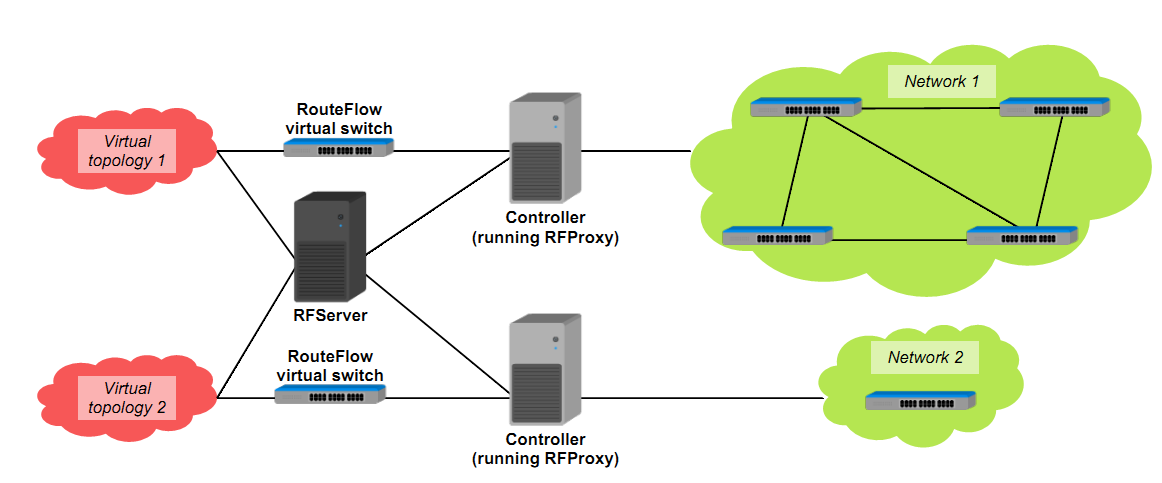
\includegraphics[width=160mm]{multiplosProxies.png}
\caption{Ambiente com inúmeros proxies e inúmeras redes.}
\label{fig:multiplosProxies} 
\end{figure}

Outro trabalho futuro será a remoção do looping infinito 
para leitura de mensagens vindas do servidor RouteFlow, 
um dos pesquisadores do Projeto RouteFlow está
desenvolvendo um mecanismo de comunicação mais ágil e
 eficaz. Esse mecanismo também deverá ser portado ao 
 novo proxy de forma a sempre se manter atualizado.

O site oficial do Projeto RouteFlow ainda descreve uma 
série de trabalhos que visam aumentar o desempenho do
sistema como um todo. Muitos exigirão a manutenção e 
atualização do proxy. Abaixo temos uma lista das principais
atualizações:

\begin{itemize}
\item \textit{Multiplexação de Roteadores:} mapeamento
de várias máquinas virtuais em um mesmo \textit{switch}
físico;
\item \textit{Aumento da Resiliência:} criação de um ambiente
de emergência que seria ativado em caso de falha do ambiente
principal;
\item \textit{Execução nas Nuvens:} execução do RouteFlow
em uma nuvens pública, como a disponibilizada pela Amazon.
\end{itemize}

